\chapter{INTRODUCTION}
\label{chapter:introduction}

\par
Software Testing is a broad field which has been researched for more than 30 years and is applied to a vast majority of software companies across the globe. According to Pretschner et. al \cite{Pretschner_MBTInPractice}, nowadays, half of the overall development resources and time are spent for quality assurance, which is the biggest motivation to optimize the testing process and minimize the time and cost of designing, developing and executing a test in order to retain the quality of the product.


\par
Brainloop, just like other companies in the field is no exception. As an organization they are mostly focused on the security and quality of their products, and spare fewer resources for testing. Including the Unit and Integration tests that are created by developers, nearly 50\% of the teams resources is utilized in testing. Brainloop has always been open to new approaches and trends for optimizing processes and is particularly interested in applying the \acrlong{mbt} (\acrshort{mbt}) approach to one of its products: an iOS application called Brainloop Secure Client (\acrshort{bsc}).

\section{Agile Scrum in Brainloop}

\par
As a process for software development Brainloop makes use of the agile scrum \cite{Agile_Scrum} model. This includes smaller agile teams that consist of a product owner, developers, quality engineers and a scrum master. The product owner is responsible for delivering well thought out and fully described requirements in the form of a User Story. The role of the developers is to completely implement the user stories comprising of the functional program code which also includes the unit and integration test codes/scripts. The quality engineers are the ones responsible for documenting the test cases in order to verify the correct implementation of the feature functionality and \acrlong{gui} according to acceptance criteria, described in the user story. They also modify/update any other previously documented test case that needs adjustments, based on new user stories. Quality engineers play an important role in the automation and execution of the manually documented test cases, while also performing exploratory tests against new features. The Scrum Master's responsibility is to find solutions to all kinds of impediments faced by the team members during the development and testing phases as well as optimizing the overall agile process within the team.

\par
The team as a whole, is responsible for the delivery of the software increment over the length of a sprint, which in case of Brainloop is 2 weeks. During the sprint, a couple of team meetings are held, which are vital for the scrum process at Brainloop. These meetings are refinement, planning, retrospective and iteration review. During the refinement meeting, product owner introduces new user stories to the team, where team members discuss points around user story, raise questions regarding it and if the team is satisfied with the provided solutions and there are no impediments regarding this specific user story, it is refined and team accepts it. Next meeting is planning, where refined user stories get estimated and based on team capacity they are included into the next sprint. During retrospective meeting team members are discussing beneficial and harmful points during the sprint and providing this information to scrum master, who is responsible for resolving harmful issues. Iteration review takes place at the end of every sprint, where all teams shown their delivered increment to other teams and management.

\section{Current Testing Process in Brainloop}

\par
During the sprint, quality engineers' work consists of duties such as documenting test cases, executing them manually and automating them as well. Documenting test cases includes analyzing the acceptance criteria of user stories included into the current sprint and documenting test cases thought by him or her into the issue tracker software. Along with this, quality engineer needs to keep track of previously documented test cases and alter those which are affected by the acceptance criteria of the new user story.

\par
After documenting test cases, quality engineer needs to execute documented test cases against \acrlong{aut} in different environments, such as different operating systems, different devices, different server versions etc. Quality engineer needs to make sure that already implemented functionality of \acrlong{aut} remains stable and it is not broken by provided increment. For this he/she needs to execute Regression test plan which usually includes majority of the documented test cases for the whole functionality of the \acrlong{aut}. In case if quality engineer finds inconsistencies between expected behaviour and actual behaviour of \acrlong{aut}, it needs to be documented in the issue tracker software as a bug. Bug needs to have clear and explicit reproduction steps, needs to include log files from \acrlong{aut} and the information about environment where it got reproduced. After the bug is fixed by developers, tester's job also includes verifying that it is not reproducible any more.

\par
According to his or her capacity, quality engineer also needs to include test automation tasks into the sprint. In scope of this task, tester needs to automate test execution with predefined test execution software or framework, verify that automated test run is stable and does not provide false positive or true negative results.

\par
To illustrate description above, current testing process looks like figure below.

\begin{figure} [htbp!]
	\centering
					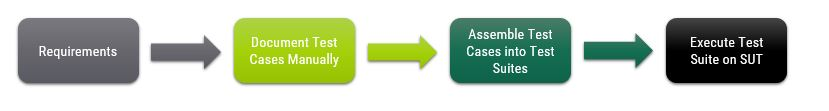
\includegraphics[width=1\textwidth]{figures/current_testing_process_flow.JPG}
					\caption{\label{Fig:current_testing_process_flow} Current Testing Process}
\end{figure}

\subsection{Pitfalls of current testing process}
\par
Even though testing process is quite fast, agile and is able to detect most of the bugs before the release, it can still be optimized by addressing the issues described below.

\par
Test cases are documented in static form, describing execution actions and expected results in plain English. They don't have any binding between each other, other than referencing, because of which similar kind of test cases involve lots of copying and pasting same text between each other, which brings up problem of their maintainability. When there is huge number of test cases which needs to be altered due to change in requirements, it takes significant time from testers' capacity to adjust these test cases to new requirements.

\par
Even if newest trends of test automation patterns, such as Keyword Driven Automation or Page Object Pattern are applied, the tester still needs to create test modules for each test case separately, which needs to be adjusted to new requirements as well when it is required. Also, each of them need to have setup and teardown modules, ensuring the predefined starting and ending state of the test. This significantly increases execution time of each test and makes it less realistic compared to real customer use.

\par
In case of UI and Functional tests it is very difficult to talk with exact numbers in terms of coverage. When testers think of possible test cases for specific user story, they do their best to examine functionality from different perspectives, with different permission sets etc. At the end, generation of test cases are bound to the creativity of every quality engineer and does not make sure that all “good” test cases (one which detects potential failure with good cost-effectiveness) are documented and executed.

\par
When there is a single unchanged regression test suite for \acrlong{aut}, which only gets incremented with test cases for new user stories, software gets resistant to this test suite and it stops finding new bugs, because all the bugs which it could have found are already fixed. This problem is known as Pesticide Paradox \cite{Pesticide_Paradox}.

\par
For addressing above mentioned issues, \acrshort{mbt} comes into the picture with opportunity to automate not only the test execution but also the test design and generation process. Therefore, company is interested to see the results and improvements regarding quality, time and cost that can be achieved with this new approach.

\par
To sum up, the goal of this thesis is to give Brainloop information based on a research and case study, which will indicate how model-based testing will fit to the company’s agile environment, whether the change from existing testing process to model-based testing will improve the software quality and will be cost-effective.

\section{Requirements}

\par
The main requirement from Brainloop is that new approach should be usable by all quality engineers in the company. As testers are mostly involved in test design and execution process, they are not obliged to be proficient with any programming language or programming basics itself. So, to translate the requirement, the chosen approach and tool for implementing \acrshort{mbt} in Brainloop needs to be as much user friendly as possible, preferably needs to have GUI for modelling and test generation as well, so that less training is needed for quality engineers to adopt \acrshort{mbt}.

\section{Model-Based Testing}

\par
Models have been applied in Software Development for already many years with different use-cases, such as describing specification, code generation etc. In our case, we apply models for describing application behaviour. Modeling is very economical way for capturing knowledge about \acrlong{aut}. This knowledge was put on the same level as gold by Apfenbaum et. al. \cite{Apfenbaum_MBT} Unlike the traditional testing process, where quality engineer needs to maintain all static test cases documented in issue tracker software, model is the only artifact which needs to be maintained for describing actions and expected results. It takes significantly less time to update model when change occurs in \acrlong{aut} compared to updating statically documented test cases. Many researchers including Pretschner \cite{Pretschner_MBTInPractice} and Apfenbaum \cite{Apfenbaum_MBT} claim that models are created anyways with different representations during traditional testing process. They are either mental models, or sketched on paper or etc. Difference is that these models are not documented explicitly. They die soon and lots of potential good test cases die with them.

\par
Another advantage which \acrshort{mbt} has over traditional testing is that it is free of ambiguous text descriptions, such as "Verify that action is handled appropriately". It is fact that different people write different test cases and information encapsulated in test case can be interpreted in many ways.

\par
Models can be created with many different paradigms, such as \acrlong{efg}, \acrlong{fsm}(\acrshort{fsm}) etc. which will be explored in next chapter, but the general flow of \acrshort{mbt} process is as described in the figure below. 


\begin{figure} [htbp!]
	\centering
					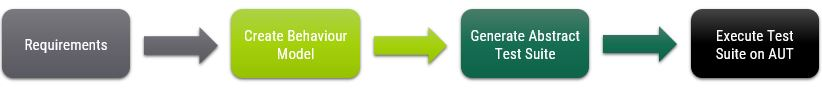
\includegraphics[width=1\textwidth]{figures/MBT_Flow.JPG}
					\caption{\label{Fig:MBT_Flow} Model-Based Testing Process}
\end{figure}

We create model, then we apply different algorithms with different coverage criteria against this model and generate abstract test cases and we execute generated test cases against \acrlong{aut}. Technically we can create one model for describing whole behaviour of application, but for complex applications, such as \acrshort{bsc}, it would become huge and unreadable. For this reason we need to apply some techniques for splitting these models, such as hierarchical modeling, or splitting models with shared steps among other small models and use flattening or similar techniques for assembling all created models before we try to apply coverage algorithms.

\par
User can apply \acrshort{mbt} in two different ways, either off-line or on-line. Both of them have their advantages and disadvantages which will be discussed in next subsections.

\subsection{Off-line Model-Based Testing}
In Off-line \acrshort{mbt}, test generation and execution are completely decoupled. One can generate test cases from model and then execute them against \acrlong{aut} with any means and in any supported environment. There are couple of advantages which off-line \acrshort{mbt} has over on-line, such as it is easier to integrate into the current testing process as it requires less changes. Generated tests can also be split and executed in parallel to save time during test execution. The most significant advantage what off-line \acrshort{mbt} has over on-line, is that it does not require automation of test execution. As automation of test execution is very extensive and time consuming implementation task, it is outside the scope of a masters thesis, so this is the main reason why we decided to proceed with off-line \acrshort{mbt} instead of on-line.

\subsection{On-line Model-Based Testing}
During on-line \acrshort{mbt} test generation and execution are coupled and happen at the same time. Unlike off-line \acrshort{mbt} it tolerates non-functional requirements. This would give the opportunity to run tests on test machines for couple of months which would ensure application exploration into millions of different ways. The generation process strongly depends on execution process which is main advantage of on-line \acrshort{mbt} over off-line.    Based on the results from execution, generation algorithms can choose different possible paths in the model. As it requires complete execution automation, it is very painful and time consuming to integrate into the current testing process, but when there is already complete test automation suite for \acrlong{aut}, on-line \acrshort{mbt} is the preferred way to go in most cases.


\section{Structure of the Thesis}
The thesis has been organized in a straightforward and effective manner to ease understanding. The flow of the thesis is described below:

\begin{enumerate}

\item \textit{Literature Review: }
Purpose of this chapter is to show investigations done for choosing the modeling approach and tool, which will fit most for the \acrshort{bsc}’s behaviour model. We review different modeling paradigms available for \acrshort{mbt} as well as the tools used by different researchers or companies to apply \acrshort{mbt} according to their needs. At the end of the chapter, justification will be provided regarding chosen paradigm and tool and how it fulfills our requirements and needs.

\item \textit{Modeling: } This chapter will provide information regarding our \acrlong{aut}, will describe the purpose of it's use and will give detailed information about modeling the behaviour of each part of the application.

\item \textit{Test Generation: } In this chapter, we will discuss different test generation criteria provided by our chosen tool, also justification will be provided about why it makes more sense to structure models in layers and also the definition of \acrshort{mrp} (\acrlong{mrp}) will be provided which was introduced in scope of this thesis.

\item \textit{Test Execution and Results: } This chapter provides information regarding execution effort of generated tests together with numbers of found issues during the test execution. Besides that, reader will find comparison of results from current testing process to our results and explanation, why some issues were detected by former testing process and not by latter as well as explanation about opposite statement.

\item \textit{Conclusion:  }In this chapter, we will summarize effort and results of applying \acrshort{mbt} for \acrshort{bsc}. We will describe the vision about how \acrshort{mbt} can be integrated into the current Scrum process in Brainloop so that transition from current testing process to \acrshort{mbt} is smooth and we will describe the lessons learned during the thesis.

\item \textit{Limitations and future work: } In this chapter, we finish this study by addressing few limitations of our testing approach. We also discuss the enhancements and improvisations that can be fulfilled regarding application of \acrshort{mbt} in the future, which regrettably could not be addressed in this thesis.

\item \textit{Appendix: } In the further chapters, we have tabulated all the terminologies used throughout the report in more detail which may not be known to a layman and a few abbreviations that have been used.
    
\end{enumerate}